%%%%%%%%%%%%%%%%%%%%%%%%%%%%%%%%%%%%%%%%%
% Laboratory Report LaTeX Template
%
% This template has been downloaded from:
% http://www.latextemplates.com
%
%%%%%%%%%%%%%%%%%%%%%%%%%%%%%%%%%%%%%%%%%

%----------------------------------------------------------------------------------------
%	DOCUMENT CONFIGURATIONS
%----------------------------------------------------------------------------------------

\documentclass{article}

\usepackage{graphicx}
\usepackage{amsmath}

\title{The Night Sky \\ ASTR 101} % Title

\author{Jordan \textsc{Ell} \\ jordan.ell7@gmail.com \\ V00660306} % Author name

\begin{document}

\maketitle % Insert the title, author and date

\begin{tabular}{lr}
Date Performed: 10/09/2012\\ % Date the experiment was performed and partner's name
Instructor: Dr. Russel Robb % Instructor/supervisor
\end{tabular}

\setlength\parindent{0pt} % Removes all indentation from paragraphs

\renewcommand{\labelenumi}{\alph{enumi}.} % Make numbering in the enumerate environment by letter rather than number (e.g. section 6)

%----------------------------------------------------------------------------------------
%	SECTION 1
%----------------------------------------------------------------------------------------

\section{Objective}

To be introduced to the essential objects of astronomy which are: planets, stars, galaxies, nebulae, and telescopes. This is
achived through observation of the night sky.\\
 
%----------------------------------------------------------------------------------------
%	SECTION 2
%----------------------------------------------------------------------------------------

\section{Equipment}

For this lab, we will be using two telescopes. The first of which will be used for deep-sky objects is the University of Victoria's 
38 inch telescope. This telescope is found in the Bob Wright Centre in the dome on the roof. The telescope is computer
controller for movement from one cellestial object to the next. The dome itself is operated sperately and needs to be 
rotated to compinsate for the telescope's direction. The second telescope we will be using is the Celestron C8 Cassegrain
telescope which is operated by a GoTo mount and is placed on the rood top.\\

We will take this time to explain the parts of the Celestron C8, as it is the telescope of most interest in this lab. All parts of the 
C8 can be found labeled in Figure~\ref{fig:telescope}. First we have the main optical tube which is a Cassegrain reflecting
telescope. The light entering the front of the tube and travels to the primary mirror. Here, the light is reflected to the
secondary mirros which again reflects the light back to the rear of the telescope and into the eyepiece.

% Telescope
\begin{figure}[h]
\centering
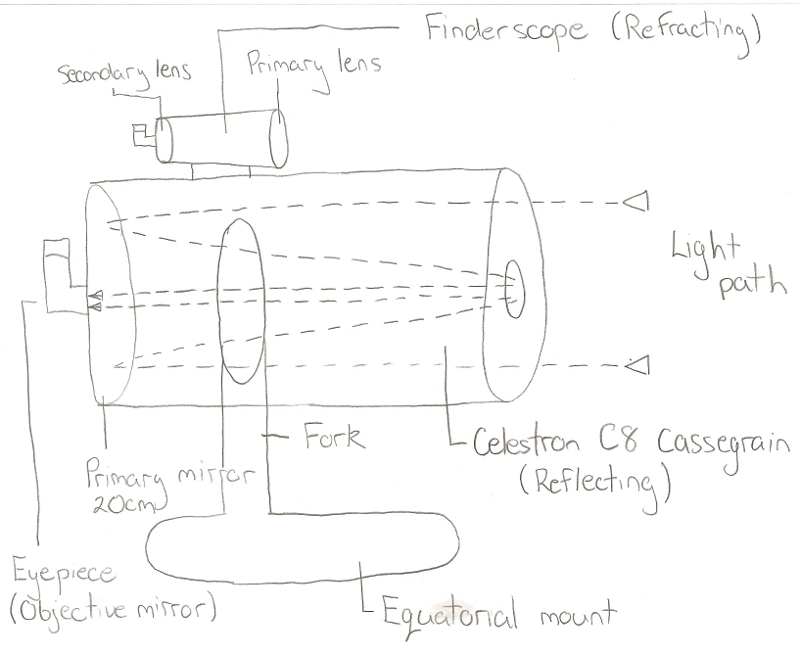
\includegraphics[width=0.7\textwidth]{images/telescope}
\caption{The Celestron C8 used in this lab.\label{fig:telescope}}
\end{figure}

Resting on top of the primary optical tube is the finderscope. The finderscope is used to align the telescope easier because of
its wider field of view. Plainly put, it is easier to get objects in the finderscope than the main optical tube because its field of
view is much wider while its magnification is lower. The finderscope is a refracting telescope as opposed to reflecting. It uses
two lenses, the primary where the light enters and the secondary where the light passes out and into the eyepiece. Refracting
telescopes use to be the main tool used for astronomy before Isaac Newton who created the first reflecting telescope in 1668
~\cite{Hall:67}.

The telescope is proped up by what is called the fork and rests on top of an equatorial mount as opposed to the altazimuth mount.\\

The equations for calculating the telescope's brightness in contrast to a human eye as well as its magnification power can be
found in Section 5 Calculations.\\

%----------------------------------------------------------------------------------------
%     SECTION 3
%----------------------------------------------------------------------------------------

\section{Procedure}

\subsection{The Constellations}
While this section of the lab is labelled "The Constellations" what we will actually be looking at is the asterisms which are the
basis for the constellations. Using the star map provided as well as being guided by the T.A, sketch three (3) new constellations
that you learnt tonight. Describe the mythology associated with each of the constellations. Learn three stars and label them 
inside of the constellation sketches and be sure to note the date, time, and weather of the observations.

\subsection{Deep-Sky Objects: Star Clusters, Bebulae, Galaxies}
Here we will look at cellestial objects which are very dim and therefore harder to see with small telescopes. Using the 
University of Victoria's 38inch telescope, locate the 3 following deep-sky objects: M11, M15, and M57. Sketch each of these
objects and be sure to note the time and date and weather conditions of each siting. Give a brief summary of what each
of these objects are.

\subsection{The Stars}
Here we will observe some interesting stars as well as look at the closest galaxy to our own Milky Way. Using the provided
Celestron C8 telescopes, locate the following three objects: Alberio, Mizar, and The Andromeda Galaxy. Sketch each one of these
and provide a brief description of each. Be sure to note the time, date, and conditions for each observation.


%----------------------------------------------------------------------------------------
%	SECTION 4
%----------------------------------------------------------------------------------------

\section{Observations}

\subsection{The Constellations}
The three asterisms observed in this part of the lab were: Cygnus, Andromeda, and Pegasus. Cygnus was observed at the time
21:00 on the night of 10/09/2012 under clear weather conditions at 48 degrees latitude and is located approximately in
the upper eastern section of the sky. A sketch of Cygnus can be found in
Figure~\ref{fig:cygnus}. Cygnus, otherwise known as the Nothern Cross, is the Greek word for swan which is represents in the sky.
Cygnus contains the star Denab which is part of the summer triangle. Cygnus also contains the famous Cygnus X-1 which is widely
believe to be a black hole for its enormous X-ray source~\cite{ESA:2012}. Cygnus in mythology, is identified with several legendary
swans; one of which is when Zeus disguised himself as a swan to seduce Leda~\cite{Tirion:2001}.

% Cygnus
\begin{figure}[h]
\centering
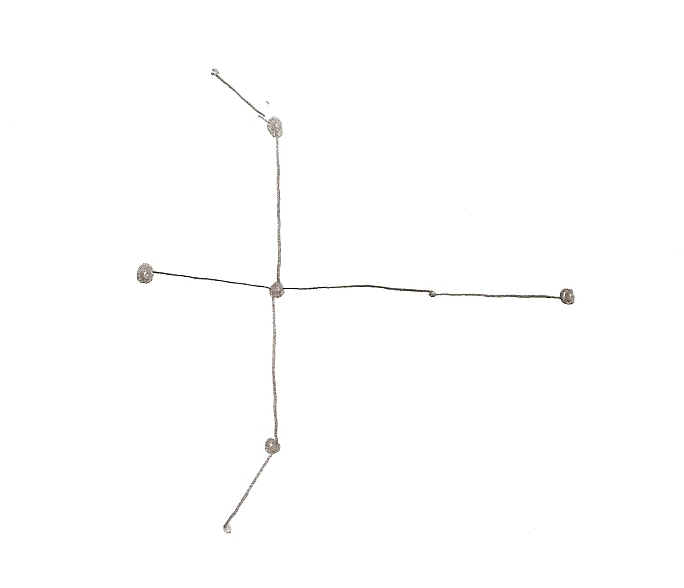
\includegraphics[width=0.5\textwidth]{images/cygnus}
\caption{The asterism of Cygnus.\label{fig:cygnus}}
\end{figure}

The asterism of Andromeda was observed at the time 21:05 of the night 10/09/2012 under clear weather conditions at 48 degrees
latitude and is located approximately in the middle eastern section of the sky. A sketch of Andromeda can be found in Figure~\ref{fig:and}.
Andromeda is involed in the mythological story of Perseus, Cepheus, and Cassiapeia in which Cassiopeia bragged that her daughter
was more beautiful than the Nereids, sea nymphs blessed with beauty. After an attack by Poseidon to punish Cassiopeia, Andromeda's
father, Cepheus, was told to sacrifice his daughter. Andromeda was later saved however by Perseus~\cite{Thompson:2007}. Andromeda
contains the binary star known as Alpheratz and is the third brightest start in the asterism~\cite{Moore:2000}.

% Andromeda
\begin{figure}[h]
\centering
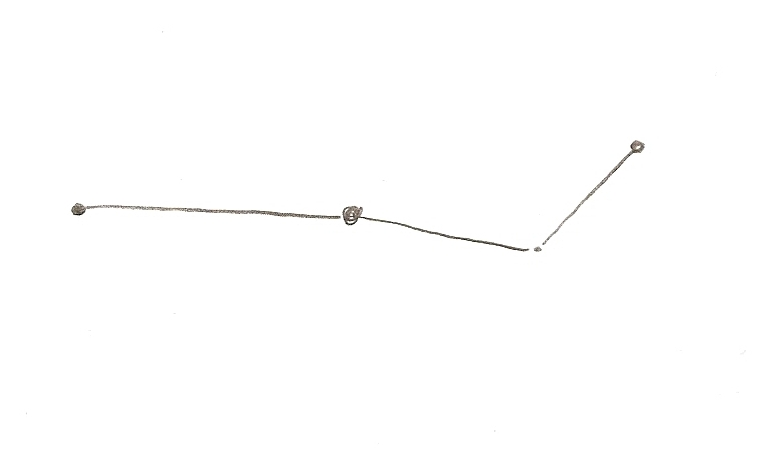
\includegraphics[width=0.5\textwidth]{images/andromeda}
\caption{The asterism of Andromeda.\label{fig:and}}
\end{figure}

The asterism of Pegasus was observed at the time 21:08 of the night 10/09/2012 under clear weather conditions at 48 degrees
latitude and is located approximately in the middle eastern section of the sky right next to Andromeda and under Cygnus. A sketch
of Pegasus can be found in Figure~\ref{fig:peg}. 51 Pegasi, a star in this constellation, was the first extrasolar Sun-like star found
to have a planet orbiting it~\cite{Mayor:1995}. Pegasus is involed is many mythological stories including how he delivered Medusa's
head to Polydectes after Perseus cut off her head.

% Pegasus
\begin{figure}[h]
\centering
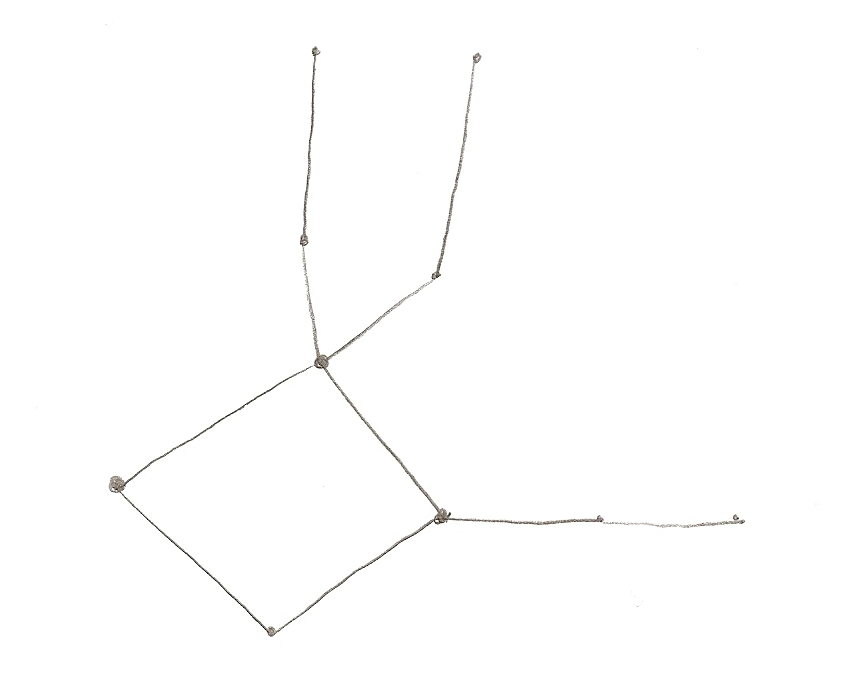
\includegraphics[width=0.5\textwidth]{images/pegasus}
\caption{The asterism of Pegasus.\label{fig:peg}}
\end{figure}

\subsection{Deep-Sky Objects: Star Clusters, Nebulae, Galaxies}

The three Messier objects observed were: M57, M15, and M11. M57, the Ring Nebula, was observed at 21:16 on the night 10/09/2012 
under clear weather conditions at 48 degrees latitude. A sketch of M57 can be found in Figure~\ref{fig:m57}. M57 appears in the
constellation of Lyra and is an example of a planetary nebula, which is an emission of ionized gas expelled during a star's late life~\cite{Soker:2009}. Planetary nebula may result from the death of intermediate and low mass stars~\cite{Costa:2009}.

% M57
\begin{figure}[h]
\centering

\includegraphics[width=0.4\textwidth]{images/blank}
\caption{The Messier 57 object.\label{fig:m57}}
\end{figure}

M15, a globular cluster, was observed at 21:23 on the night 10/09/2012 under clear weather conditions at 48 degrees latitude. A sketch
of M15 can be found in Figure~\ref{fig:m15}. M15 can be described as a large gathering of star which the brighter are more often 
located towards the centre of the cluster while the dimmer appear towards the outer rim. M15 in particular is thought to have a 
black hole located at its centre~\cite{Marel:2003}.

% M15
\begin{figure}[h!]
\centering

\includegraphics[width=0.4\textwidth]{images/blank}
\caption{The Messier 15 object.\label{fig:m15}}
\end{figure}

M11, an open cluster, was observed at 21:30 on the night 10/09/2012 under clear weather conditions at 48 degrees latitude. A sketch
of M11 can be found in Figure~\ref{fig:m11}. M11 can be described as a large cluster of stars, however, not all brightest stars appear
at the centre of the cluster. Star appear to be randomly spread out inside of the cluster. It is believed that its more or less triangular
shape is similar to that of a flock of flying ducks.

% M11
\begin{figure}[h]
\centering

\includegraphics[width=0.5\textwidth]{images/blank}
\caption{The Messier 11 object.\label{fig:m11}}
\end{figure}

\subsection{The Stars}

The two stars observed were Mizar/Alcor and Alberio in addition to the Andromeda Galaxy being observed. The stars Mizar and Alcor
were observed at 21:32 on the night 10/09/2012 under clear weather conditions at 48 degrees latitude. A sketch of the stars can be 
found in the Figure~\ref{fig:mizar}.

% mizar
\begin{figure}[h!]
\centering
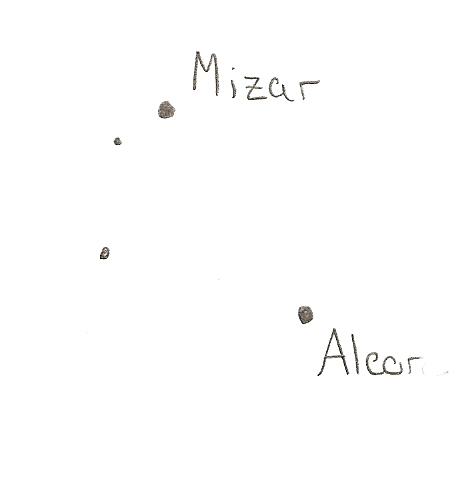
\includegraphics[width=0.4\textwidth]{images/Mizar}
\caption{The stars Mizar and Alcor.\label{fig:mizar}}
\end{figure}

The star Alberio was observed at 21:40 on the night 10/09/2012 under clear weather conditions at 48 degrees latitude. A sketch of the 
star can be found in Figure~\ref{fig:alberio}. Alberio contains two stars. The left star shines a red colour while the right star shines blue.
The star that shines blue must be hotter because blue is a more energetic end of the light spectrum which means that is must be
generating more energy than the red one.

%Alberio
\begin{figure}[h!]
\centering
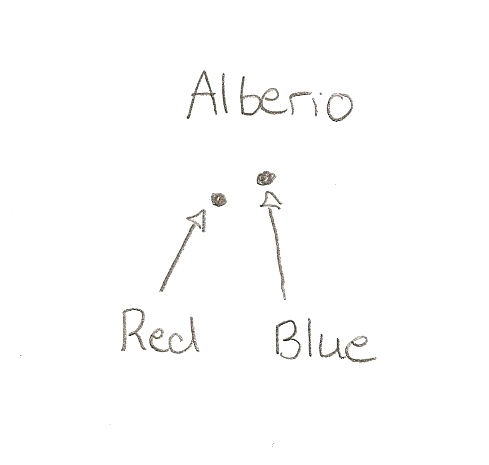
\includegraphics[width=0.4\textwidth]{images/alberio}
\caption{The stars of Alberio.\label{fig:alberio}}
\end{figure}

The Andromeda Galaxy was observed at 21:49 on the night 10/09/2012 under clear weather conditions at 48 degrees latitude. A
sketch of the galaxy can be found in Figure~\ref{fig:andg}. The Andromeda Galaxy can be described as an elliptical blur in the sky
where its centre is more concentrated than the perimeters. The Andromeda Galaxy is actually the closet galaxy to our own 
Milky Way at about 2.5 million light-years from Earth~\cite{Ribas:2005}. The Andromeda Galaxy is also part of the Messier objects and is known as M31.

% AndromedaG
\begin{figure}[h!]
\centering
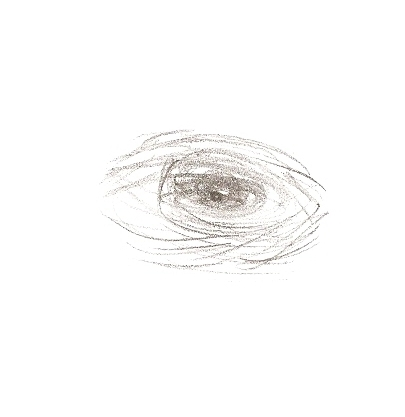
\includegraphics[width=0.5\textwidth]{images/andromedagalaxy}
\caption{The Andromeda Galaxy. Also known as M31\label{fig:andg}}
\end{figure}


%----------------------------------------------------------------------------------------
%	SECTION 5
%----------------------------------------------------------------------------------------

\section{Calculations}

For the light gathering abilities of the Celestron C8 telescope, let us contrast it to that of the human eye. The pupil in the eye is used for
gathering light and is on average about 1cm in diameter. The primary mirror of the C8 is also used for light gathering and has 
the diameter of 20cm.  The equation for area of a circle is shown in Equation~\ref{eq:area} below. We can use this to calculate the ratio of the
telescope's primary mirror to that of the human eye in Equation~\ref{eq:bri}.

\begin{equation} \label{eq:area}
A = \pi * r^2
\end{equation}
\begin{equation} \label{eq:bri}
{\frac{A_m}{A_e}} = {\frac{\pi * 10cm^2}{\pi * .5cm^2}} = 400
\end{equation}

From Equation 2 above we see that the C8 has 400 times the light gathering ability as compared to the human eye. Now as for
magnification, we look to Equation~\ref{eq:mag}. We see here that the magnification is equal to the focal length (f) of the primary
mirror divided by the focal length of the objective mirror.

\begin{equation} \label{eq:mag}
m = {\frac{f_p}{f_o}} = {\frac{2000mm}{40mm}} = 50
\end{equation}

From Equation~\ref{eq:mag}, we see that magnification is 50 times.\\


%----------------------------------------------------------------------------------------
%	SECTION 6
%----------------------------------------------------------------------------------------

\section{Evaluation}
Overall, I liked the lab as a refresher to the night sky. I had lots of previous knowledge of the constellations and of some key Messier
objects and what they were, however I was never able to view them through my own telescope. The most I took away was some of
the mythology from the constellations as I had never researched it on my own.


%----------------------------------------------------------------------------------------
%	BIBLIOGRAPHY
%----------------------------------------------------------------------------------------

\begin{thebibliography}{9}

\bibitem{Hall:67}
Isaac Newton: adventurere in thought, by Alfred Ruper Hall, page 67.
\bibitem{ESA:2012}
Staff (2004-11-05), Observations: Seeing in X-ray wavelengths, ESA, retrieved 2008-08-12.
\bibitem{Tirion:2001}
Ridpath and Tirion 2001, pp. 134-137.
\bibitem{Thompson:2007}
Thompson and Thompson 2007, pp. 66 to 73.
\bibitem{Moore:2000}
Moore 2000, pp. 328 to 330.
\bibitem{Mayor:1995}
Mayor, Michael; Queloz, Didier (1995). "A Jupiter-mass companion to a solar-type star". Nature 378 (6555): 355 to 359.
\bibitem{Soker:2009}
Frankowski and Soker 2009.
\bibitem{Costa:2009}
Maciel, Costa and Idiart 2009, pp. 127 to 37.
\bibitem{Marel:2003}
Gerssen, J; van der Marel, R P; Gebhardt, K; Guhathakurta, P; Peterson, R C; Pryor, C (2003).
\bibitem{Ribas:2005}
Ribas, I. et al. (2005). "First Determination of the Distance and Fundamental Properties of an Eclipsing Binary in the Andromeda Galaxy". Astrophysical Journal Letters 635 (1): L37 to L40

\end{thebibliography}

\end{document}